%%%%%%%%%%%%%%%%%%%%%%%%%%%%%%%%%%%%%%%%%%%%%%%%%%%%%%%%%%%%%%%%%%
%%%%%%%%%%%%%%%%%%%%%%%%%%%%%%%%%%%%%%%%%%%%%%%%%%%%%%%%%%%%%%%%%%
% \setmathfont{TeX Gyre Termes Math}
%Packages
\documentclass[10pt, a4paper]{article}
\usepackage[top=3cm, bottom=4cm, left=2cm, right=2cm]{geometry}
\usepackage{amsmath,amsthm,amsfonts,amssymb,amscd, fancyhdr, color, comment, graphicx, environ}
\usepackage{float}
\usepackage{booktabs}
\usepackage{pifont}
\usepackage{mathrsfs}
\usepackage[math-style=ISO]{unicode-math}
\usepackage{lastpage}
\usepackage[dvipsnames]{xcolor}
\usepackage[framemethod=TikZ]{mdframed}
\usepackage{enumerate}
\usepackage[shortlabels]{enumitem}
\usepackage{fancyhdr}
\usepackage{indentfirst}
\usepackage{listings}
\usepackage{sectsty}
\usepackage{thmtools}
\usepackage{shadethm}
\usepackage{hyperref}
\usepackage{setspace}
\usepackage{adjustbox}
\hypersetup{
    colorlinks=true,
    linkcolor=blue,
    filecolor=magenta,      
    urlcolor=blue,
}
\usepackage{xcolor,colortbl}
%%%%%%%%%%%%%%%%%%%%%%%%%%%%%%%%%%%%%%%%%%%%%%%%%%%%%%%%%%%%%%%%%%
%%%%%%%%%%%%%%%%%%%%%%%%%%%%%%%%%%%%%%%%%%%%%%%%%%%%%%%%%%%%%%%%%%
%Environment setup
\mdfsetup{skipabove=\topskip,skipbelow=\topskip}
\newrobustcmd\ExampleText{%
An \textit{inhomogeneous linear} differential equation has the form
\begin{align}
L[v ] = f,
\end{align}
where $L$ is a linear differential operator, $v$ is the dependent
variable, and $f$ is a given non−zero function of the independent
variables alone.
}
\mdfdefinestyle{theoremstyle}{%
linecolor=black,linewidth=1pt,%
frametitlerule=true,%
frametitlebackgroundcolor=gray!20,
innertopmargin=\topskip,
}
\mdtheorem[style=theoremstyle]{Problem}{Question Number}
\setcounter{Problem}{4}
\newenvironment{Solution}{\textbf{Solution.}}

\definecolor{codegreen}{rgb}{0,0.6,0}
\definecolor{codegray}{rgb}{0.5,0.5,0.5}
\definecolor{codepurple}{rgb}{0.58,0,0.82}
\definecolor{backcolour}{rgb}{0.95,0.95,0.92}

\lstdefinestyle{mystyle}{
    backgroundcolor=\color{backcolour},   
    commentstyle=\color{codegreen},
    keywordstyle=\color{magenta},
    numberstyle=\tiny\color{codegray},
    stringstyle=\color{codepurple},
    basicstyle=\ttfamily\footnotesize,
    breakatwhitespace=false,         
    breaklines=true,                 
    captionpos=b,                    
    keepspaces=true,                 
    numbers=left,                    
    numbersep=5pt,                  
    showspaces=false,                
    showstringspaces=false,
    showtabs=false,                  
    tabsize=2
}

\lstset{style=mystyle}
%%%%%%%%%%%%%%%%%%%%%%%%%%%%%%%%%%%%%%%%%%%%%%%%%%%%%%%%%%%%%%%%%%
%%%%%%%%%%%%%%%%%%%%%%%%%%%%%%%%%%%%%%%%%%%%%%%%%%%%%%%%%%%%%%%%%%
%Fill in the appropriate information below
\newcommand{\norm}[1]{\left\lVert#1\right\rVert}     
\newcommand\course{XXXX0000}                            % <-- course name   
\newcommand\hwnumber{0}                                 % <-- homework number
\newcommand\Information{Someone}                        % <-- personal information
%%%%%%%%%%%%%%%%%%%%%%%%%%%%%%%%%%%%%%%%%%%%%%%%%%%%%%%%%%%%%%%%%%
%%%%%%%%%%%%%%%%%%%%%%%%%%%%%%%%%%%%%%%%%%%%%%%%%%%%%%%%%%%%%%%%%%
%Page setup
\pagestyle{fancy}
\headheight 35pt
\lhead{\today \hspace*{4cm} Key-Breakers}
\rhead{
\includegraphics[width=1.2cm]{../logo.png}}
\lfoot{}
\pagenumbering{arabic}
\cfoot{\small\thepage}
\rfoot{}
\headsep 1.2em
\renewcommand{\baselinestretch}{1.25}
%%%%%%%%%%%%%%%%%%%%%%%%%%%%%%%%%%%%%%%%%%%%%%%%%%%%%%%%%%%%%%%%%%
%%%%%%%%%%%%%%%%%%%%%%%%%%%%%%%%%%%%%%%%%%%%%%%%%%%%%%%%%%%%%%%%%%
%Add new commands here
\renewcommand{\labelenumi}{\alph{enumi})}
\newcommand{\Z}{\mathbb Z}
\newcommand{\R}{\mathbb R}
\newcommand{\Q}{\mathbb Q}
\newcommand{\NN}{\mathbb N}
\newcommand{\PP}{\mathbb P}
\DeclareMathOperator{\Mod}{Mod} 
\renewcommand\lstlistingname{Algorithm}
\renewcommand\lstlistlistingname{Algorithms}
\def\lstlistingautorefname{Alg.}
\newtheorem*{theorem}{Theorem}
\newtheorem*{lemma}{Lemma}
\newtheorem{case}{Case}
\newcommand{\assign}{:=}
\newcommand{\infixiff}{\text{ iff }}
\newcommand{\nobracket}{}
\newcommand{\backassign}{=:}
\newcommand{\tmmathbf}[1]{\ensuremath{\boldsymbol{#1}}}
\newcommand{\tmop}[1]{\ensuremath{\operatorname{#1}}}
\newcommand{\tmtextbf}[1]{\text{{\bfseries{#1}}}}
\newcommand{\tmtextit}[1]{\text{{\itshape{#1}}}}

\newenvironment{itemizedot}{
    \begin{itemize} 
    \renewcommand{\labelitemi}{$\bullet$}
    \renewcommand{\labelitemii}{$\bullet$}
    \renewcommand{\labelitemiii}{$\bullet$}
    \renewcommand{\labelitemiv}{$\bullet$}}
    {\end{itemize}}

\catcode`\<=\active\def<{
\fontencoding{T1}\selectfont\symbol{60}\fontencoding{\encodingdefault}}
\catcode`\>=\active\def>{
\fontencoding{T1}\selectfont\symbol{62}\fontencoding{\encodingdefault}}
\catcode`\<=\active\def<{
\fontencoding{T1}\selectfont\symbol{60}\fontencoding{\encodingdefault}}

%%%%%%%%%%%%%%%%%%%%%%%%%%%%%%%%%%%%%%%%%%%%%%%%%%%%%%%%%%%%%%%%%%
%%%%%%%%%%%%%%%%%%%%%%%%%%%%%%%%%%%%%%%%%%%%%%%%%%%%%%%%%%%%%%%%%%
%Begin now!



\begin{document}
%%%%%%%%%%%%%%%%%%%%%%%%%%%%%%%%%%%%%%%%%%%%%%%%%%%%%%%%%%%%%%%%%%
%%%%%%%%%%%%%%%%%%%%%%%%%%%%%%%%%%%%%%%%%%%%%%%%%%%%%%%%%%%%%%%%%%
%Start the assignment now
%%%%%%%%%%%%%%%%%%%%%%%%%%%%%%%%%%%%%%%%%%%%%%%%%%%%%%%%%%%%%%%%%%
%New problem
\newpage
\begin{Problem}

\textbf{Block Cipher Cryptanalysis}

Recall the experiments from Chapter 6 of the “The Block Cipher Companion Book” discussed
in class.
\begin{itemize}
\item Implement Sypher0041
\item Use random keys using openssl rand

      – (Six 16-bits keys → k0 , · · · , k5 )
\item Verify the following experiments from the book using your implementation of Sypher004.
\item Use 6 sets of randomly generated keys.
\item Submit the well commented code so that your results can be verified.
\item Also document (preferably in a table) the randomly generated keys used here.
\item Write paragraphs for each one to describe your observations referring to the figures below.

\begin{center}
    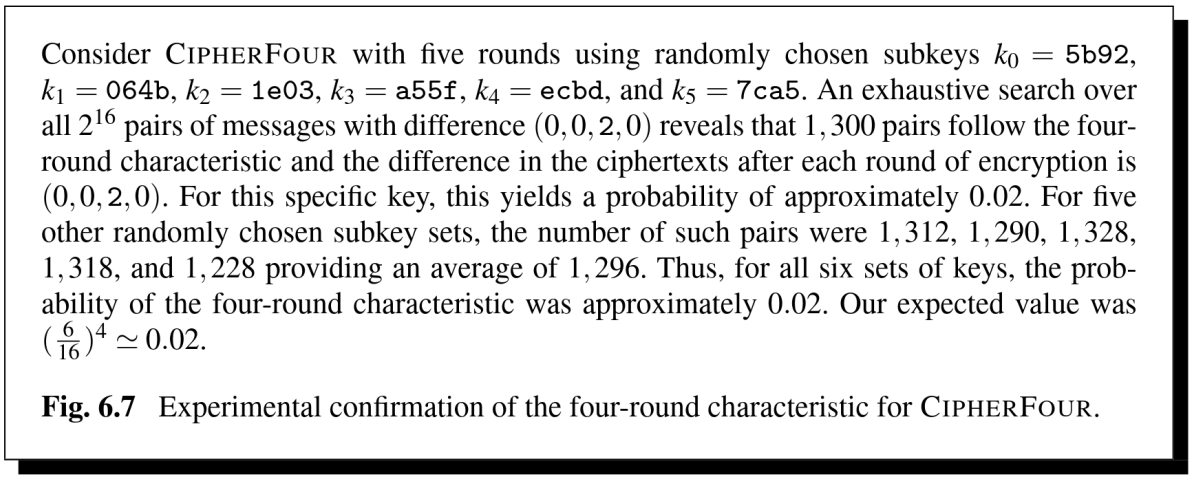
\includegraphics[width=15.2cm]{./images/q5_1.png}    
    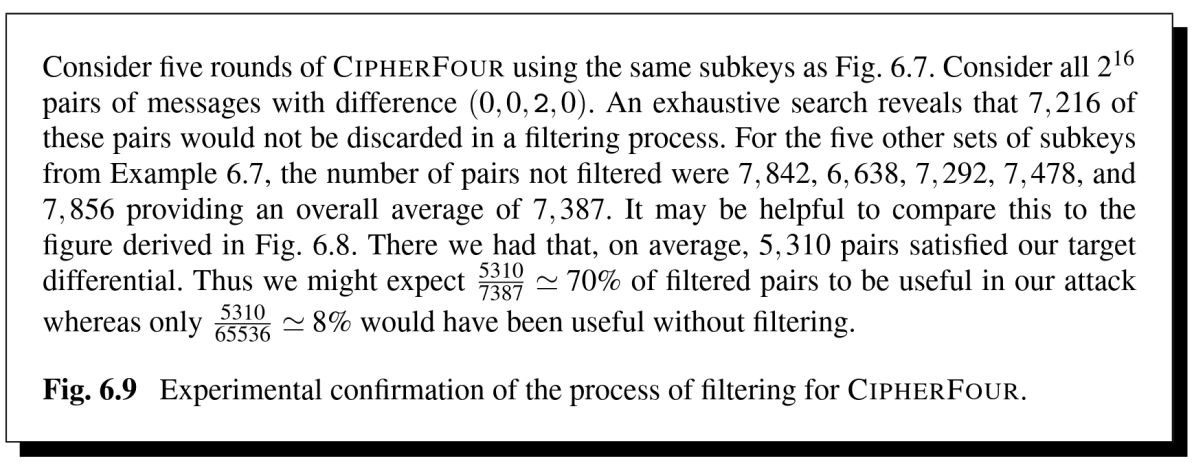
\includegraphics[width=15.2cm]{./images/q5_2.png}    
    \pagebreak
\end{center}
\begin{center}
    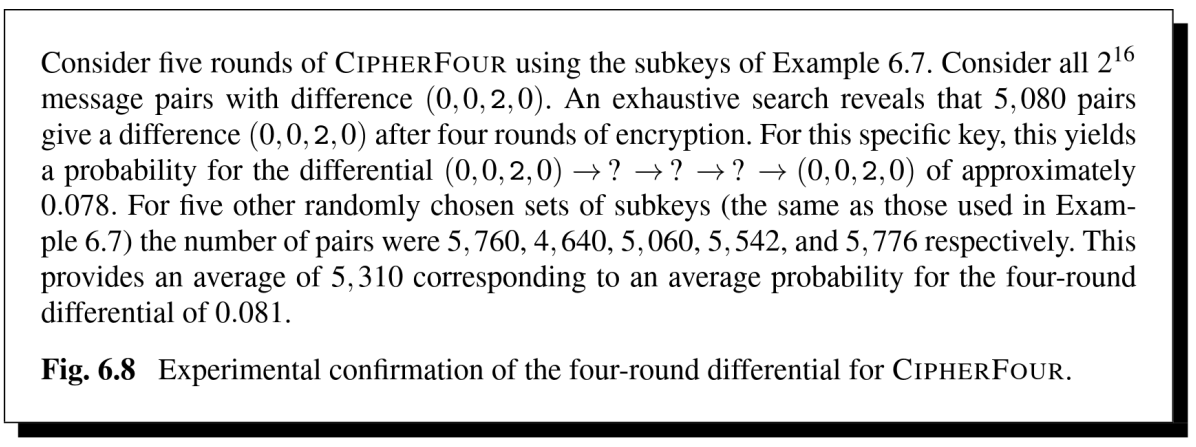
\includegraphics[width=15.2cm]{./images/q5_3.png}    
\end{center}

\end{itemize}
\end{Problem}

\begin{Solution}


The results of cryptanalysis experiment on a 4-round block
cipher, Sypher004, as described in Chapter 6 of \textit{The Block Cipher
Companion}. The experiments verify the theoretical probabilities of various
ciphertext characteristics after multiple rounds of encryption, using randomly
generated subkeys. Three key experiments were conducted, and the results are
analyzed and compared with theoretical expectations.\\


\textbf{Code Overview}
    \begin{itemize} 
        \item \textbf{sypher004.py}: 
        this file contains the implementation of Sypher004 using \texttt{S\_Box}
        and \texttt{P\_Box}. Implementation done in \texttt{Sypher004} function
        which is returning all round output as we need it in experiments by
        taking message and key\_list as argument. So to get ciphertext
        corresponding to message given in input to function, we need to take the last
        of item of the list return by the function.

        \item \textbf{utils.py}: 
        This files mainly contain the utility function as follows: -
        \begin{enumerate}
            \item \texttt{generate\_message\_pairs}: This will create $2^{16}$ a message pair with difference $(0,0,2,0)$.
            \item \texttt{generate\_random\_keys}: This function will create random 6 keys of width 16 bits with \texttt{openssl}
            \item \texttt{printResult}: This function will print data in the form of table 
        \end{enumerate}


        \item \textbf{perfrom\_all\_experiments.py}: 
        This is main file where all individual experiment called through
        respective file and will run simultaneously. Observe the output 
        of this file for all experiments.
    \end{itemize}

\pagebreak
\subsection*{Experiment 1: Verification of 4-Round Characteristic (Figure 6.7)}

The first experiment aims to confirm that pairs of messages with an initial
difference  $(0, 0, 2, 0)$follow the same difference after each round
of encryption in Sypher004.
Specifically, we want to verify that the difference
between the ciphertexts remains $(0, 0, 2, 0)$ after all four rounds.

\begin{itemize}
    \item \textbf{Code Overview}
    The file \texttt{experiment\_6\_7.py} contains all code for this experiment.
    First, it will get all round outputs as an array and then check the output difference in each round is (0,0,2,0) along with ciphertext.
    And if the condition is getting satisfied, then increasing count variable.
    Like this, iterating all over $2^{16}$ message pairs returning a result
    as count, probabilities and corresponding key list.

    Theoretically number of message pair follow this conditions should $(\frac{6}{16})^4 \times (2^{16})$ which is nearly $1300$

    \item \textbf{output}
    \begin{center}
    \begin{tabular}{|c|c|c|}
    \hline
    \textbf{Keys} & \textbf{Count} & \textbf{Probability} \\
    \hline
    64437, 33722, 19244, 46340, 3188, 62559 & 1250 & 0.0190735 \\
    \hline
    31002, 3702, 670, 23592, 4855, 24504 & 1238 & 0.0188904 \\
    \hline
    62952, 17637, 38544, 13991, 48597, 11565 & 1366 & 0.0200435 \\
    \hline
    21389, 34641, 9511, 8598, 23721, 5167 & 1228 & 0.0187378 \\
    \hline
    5091, 23723, 40716, 20399, 12796, 41693 & 1222 & 0.0186462 \\
    \hline
    256, 23770, 7796, 50154, 21357, 34062 & 1246 & 0.0190125 \\
    \hline
    \textbf{Average} & 1258.33 & 0.0192006 \\
    \hline
    \end{tabular}
    \end{center}
    \item \textbf{Observation}
    The results align with the theoretical probability of approximately $0.02$.
    For each set of random subways, around 1300 message pairs followed the
    expected characteristic, confirming the expected differential cryptanalysis
    behavior for the 4-round block cipher.

    \item \textbf{Output Image}
    \begin{center}
        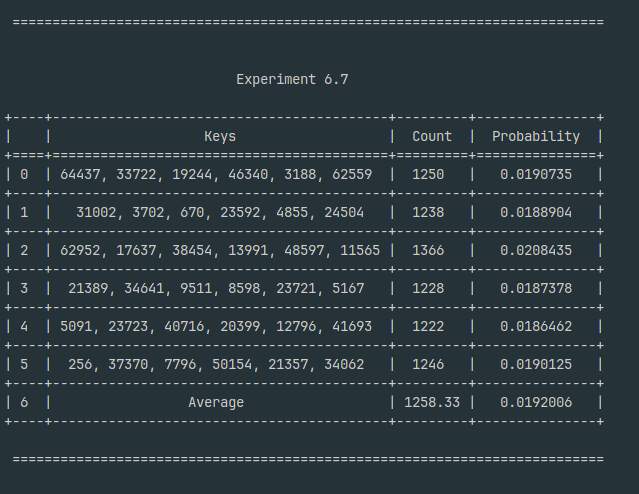
\includegraphics[width=10.2cm]{./images/Exp_6_7.png}    
    \end{center}
\end{itemize}

\pagebreak
\subsection*{Experiment 2: Verification of 4-Round Differential (Figure 6.8)}

The second experiment verifies the probability that pairs of messages with an
input difference  $(0, 0, 2, 0)$will have the same difference after four
rounds of encryption.
The Difference is here, we are not caring about the difference in
intermediate rounds.
So this is Possible in 4 ways as described in a book.

Theoretically, the number of message pairs following these conditions should be
$4 \times (\frac{6}{16})^4 \times (2^{16})$ which is nearly equal to $5200$

\begin{itemize}
\item \textbf{Code Overview}
    The file \texttt{experiment\_6\_8.py} contains all code for this experiment.
    First, it will get all round outputs as an array and then check the output
    difference only in the last round (0,0,2,0).
    And if the condition is getting satisfied, then increasing count variable.
    Like this, iterating all over $2^{16}$ message pairs returning a result as count, probabilities and
    corresponding key list.
    
    The function \texttt{isOutDiff\_2} checks whether the output difference
    between two rounds is $(0, 0, 2, 0)$ (hexadecimal difference of $32$). The
    experiment runs over $2^{16}$ message pairs for each of six sets of keys.

\item \textbf{Output}    

The results for six sets of keys are shown in the Table.
The probability is calculated as the ratio of the valid pairs to the total number of pairs.
    \begin{center}

    \begin{tabular}{|c|c|c|}
    \hline
    \textbf{Keys} & \textbf{Count} & \textbf{Probability} \\
    \hline
    1474, 23699, 38149, 51313, 30437, 33349 & 5440 & 0.0830078 \\
    \hline
    21320, 19275, 33131, 14885, 13137, 43584 & 5076 & 0.0774536 \\
    \hline
    61915, 53788, 32765, 17876, 62732, 41017 & 5074 & 0.0774231 \\
    \hline
    39045, 64900, 51936, 18716, 53674, 3330 & 5086 & 0.0776062 \\
    \hline
    27291, 27509, 55369, 26288, 60552, 62670 & 5278 & 0.0805359 \\
    \hline
    20236, 64326, 30870, 55177, 23683, 32863 & 4960 & 0.0756834 \\
    \hline
    \textbf{Average} & 5152.33 & 0.0786184 \\
    \hline
    \end{tabular}
    \end{center}

\item \textbf{Observation}
The probability of the differential being followed after four rounds is
approximately $0.081$, matching the theoretical expectations.
This confirms that for the 4-round Sypher004, the differential propagates with an approximate
probability of $0.08$.

\item \textbf{Output Image}

\begin{center}
    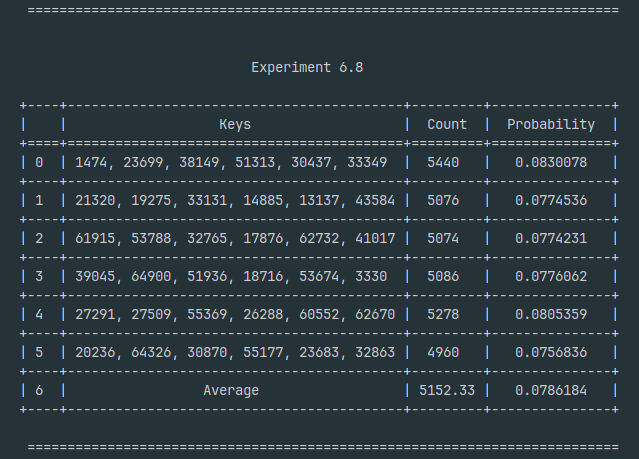
\includegraphics[width=8.2cm]{./images/Exp_6_8.png}    
\end{center}

\end{itemize}

\pagebreak
\subsection*{Experiment 3: Filtering Process Verification (Figure 6.9)}

This experiment examines how many pairs of messages survive the filtering
process during a cryptanalysis attack based on their output differences.

Theoretically number of message pairs follow these conditions should be
around $7200$

\begin{itemize}
\item \textbf{Code Overview}
    The file \texttt{experiment\_6\_9.py} contain all code for this experiment.
    First, it will get all ciphertext outputs and then check output is in format
    $(0,0,*,0)$ where $*\epsilon (1,2,9,a)$.
    And if condition is getting satisfied then increasing count variable.
    Like this, iterating all over $2^{16}$ message pairs returning a result as count, probabilities and
    corresponding key list.  

    The function \texttt {filterMessage} applies a filtering condition based on
    the differences between the ciphertexts.
    The experiment checks which pairs of messages pass the filter after five rounds of encryption.

    \item \textbf{Output}
    \begin{center}
    \begin{tabular}{|c|c|c|}
    \hline
    \textbf{Keys} & \textbf{Count} & \textbf{Probability} \\
    \hline
    45273, 31888, 29580, 60063, 421, 58621 & 7534 & 0.11496 \\
    \hline
    47578, 37394, 23143, 47900, 32957, 42989 & 6968 & 0.106323 \\
    \hline
    52646, 49922, 33642, 49306, 42176, 4233 & 6624 & 0.101074 \\
    \hline
    35029, 34852, 24598, 3156, 31122, 38511 & 7778 & 0.118683 \\
    \hline
    33964, 8177, 39554, 24457, 64005, 36912 & 7302 & 0.11142 \\
    \hline
    437, 30823, 33402, 22592, 50225, 5999 & 7696 & 0.117432 \\
    \hline
    \textbf{Average} & 7317 & 0.111649 \\
    \hline
    \end{tabular}
    \end{center}


\item \textbf{Observation}
The average number of message pairs that pass the filter is $7317$, representing
about $11.16\%$ of the total pairs.
Compared to Experiment 2, where $5152$ pairs followed the target differential, the filtering process retains approximately
$70.4\%$ of the useful message pairs.

\item \textbf{Output Image}

\begin{center}
    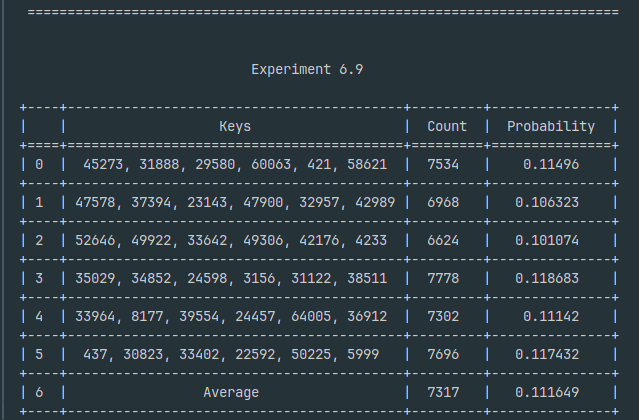
\includegraphics[width=10.2cm]{./images/Exp_6_9.png}    
\end{center}

\end{itemize}

\pagebreak
\section*{Conclusion}
The results from all three experiments confirm the theoretical probabilities for
differential cryptanalysis on the Sypher004 block cipher.
The experiments verify the expected behavior of message pairs after four rounds of encryption,
demonstrating how filtering can improve the efficiency of a cryptanalysis
attack. 
\end{Solution}

%%%%%%%%%%%%%%%%%%%%%%%%%%%%%%%%%%%%%%%%%%%%%%%%%%%%%%%%%%%%%%%%%%
%Complete the assignment now
\end{document}

%%%%%%%%%%%%%%%%%%%%%%%%%%%%%%%%%%%%%%%%%%%%%%%%%%%%%%%%%%%%%%%%%%
%%%%%%%%%%%%%%%%%%%%%%%%%%%%%%%%%%%%%%%%%%%%%%%%%%%%%%%%%%%%%%%%%%